% VLDB template version of 2020-08-03 enhances the ACM template, version 1.7.0:
% https://www.acm.org/publications/proceedings-template
% The ACM Latex guide provides further information about the ACM template

\documentclass[sigconf, nonacm]{acmart}
\usepackage{caption}
\usepackage{subcaption}
%% The following content must be adapted for the final version
% paper-specific
\newcommand\vldbdoi{XX.XX/XXX.XX}
\newcommand\vldbpages{XXX-XXX}
% issue-specific
\newcommand\vldbvolume{14}
\newcommand\vldbissue{1}
\newcommand\vldbyear{2020}
% should be fine as it is
\newcommand\vldbauthors{\authors}
\newcommand\vldbtitle{\shorttitle} 
% leave empty if no availability url should be set
\newcommand\vldbavailabilityurl{https://github.com/Lennart97/nlp_project}
% whether page numbers should be shown or not, use 'plain' for review versions, 'empty' for camera ready
\newcommand\vldbpagestyle{plain} 

\begin{document}
\title{Predicting political views based on tweets}

%%
%% The "author" command and its associated commands are used to define the authors and their affiliations.
\author{Florian Siepe}
\affiliation{%
  \institution{Philipps University of Marburg}
  \city{Marburg}
  \state{Germany}
}
\email{Siepe@students.uni-marburg.de}

\author{Lennart Hallenberger}
\affiliation{%
	\institution{Philipps University of Marburg}
	\city{Marburg}
	\state{Germany}
}
\email{Hallenb@students.uni-marburg.de}

%%
%% The abstract is a short summary of the work to be presented in the
%% article.
\begin{abstract}
In this work we discuss and evaluated an topic modeling approach towards predicting political views of users based on their tweets. For this we use a dataset which contains tweets of U.S American politicians with their respective party (Democrat or Republican) which they belong to. After cleaning and preprocessing the tweets they are embedded using an LDA model based on their topics. With these embeddings classifiers are trained to predict a political party based on a tweets. Our results show that no reliably predictions can be made with this embedding technique.
\end{abstract}

\maketitle

%%% do not modify the following VLDB block %%
%%% VLDB block start %%%
\ifdefempty{\vldbavailabilityurl}{}{
\vspace{.3cm}
\begingroup\small\noindent\raggedright\textbf{PVLDB Artifact Availability:}\\
The source code, data, and/or other artifacts have been made available at \url{\vldbavailabilityurl}.
\endgroup
}
%%% VLDB block end %%%

\section{Introduction}
\label{sec:intro}
Over the past years social media has become more relevant in politics. Not
only are politicians them self’s using social media to gain a growing following,
it’s also where citizens discuss and share their opinion on political topics.

From this comes an interest to classify social media posts by their political
point of view. One use case can be to gain insights on political topics and
their distribution amongst voters. Furthermore analyzing posts in a large
scale can play a roll in more accurate projections of future elections.

The goal of this project is to classify users based on their social media posting
in regard of their political viewpoint to match them with a political party. To test the precision and recall of our approach we use tweets made by
members of the republican and democratic party from the United States (\ref{sec:data}).
Next we apply an Latent Dirichlet allocation model (LDA) and train a classifier on these tweets to predict the party based on the tweets content (\ref{sec:app}). The results from the classifer are then evaluated and discussed (\ref{sec:eval}). Finally, we give a summary and point out the key findings of our work (\ref{sec:summ}).

\section{Dataset}
\label{sec:data}
The used dataset \footnote{@Lennart falls du die URL noch hast, bitte einfügen \url{URL}} consists out of 84502 tweets from may 2018. These tweets are collected from 433 accounts, whose owner are validated members of either the Democratic (49\%) or Republican party (51\%).

For each of these accounts, the last 200 tweets are collected with their timestamp as well as the associated owner account and the corresponding political party.

\section{Approach}
\label{sec:app}
The approach we use to predict the closeness to a specific political party consists of four main steps :

\begin{enumerate}
	\item Data cleaning
	\item Preprocessing
	\item LDA-Model building
	\item Classifier training
\end{enumerate}

\begin{figure}
	\centering
	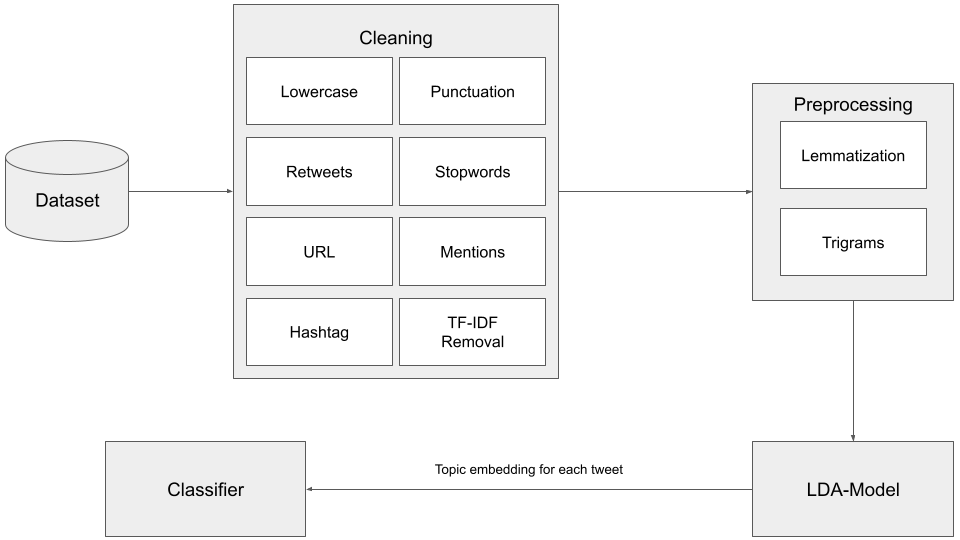
\includegraphics[width=\linewidth]{figures/pipeline}
	\caption{Pipeline of the approach}
	\label{fig:pipeline}
\end{figure}

Fig. \ref{fig:pipeline} illustrates this process. In the following each of those steps will be outlined in greater detail.

\subsection{Data cleaning}
\label{subsec:clean}
As tweets are usually noisy in terms of being grammatically correct and often contain human errors like typos, cleaning data from this noise is an essential step.

The cleaning is organized in different modules, each responsible to deal with a certain aspect of the data.

\paragraph{Lowercase} To avoid unnecessary ambiguity, all tokens are lowercased.

\paragraph{Punctuation} Special punctuation characters are remove, as they do not carry semantic meaning.

\paragraph{Stopword} The same applies to stopwords like "a" or "the". Therefore, these are being removed too.

\paragraph{Retweets} Retweets are a particular property of tweets such that a user repeats a tweets from a different user. However, since it can usually be assumed that retweeting means confirmation with the original tweets, only the respective marker is removed.

\paragraph{URL} Often users provide links to external resources in their tweets. Since extracting topics from these resources is out of scope of this project, they are simply be ignored.

\paragraph{Mentions} Twitter user can mention other users. For further improvements this information might be included to strengthen or weaken an existing classification based on the user political party (if it is known)
\paragraph{Hashtag} Similarly linke mentions, hashtags express that the tweet is relevant for a specific topic and might have an influence on the result.

\paragraph{TF-IDF} Some tokens (or words) appear only a few times, while others occur quite often. Either way, this commonly mean that these tokens are too specific and might lead to noise in the data or they do not carry much meaning. Therefore they might be removed.

\subsection{Preprocessing}
\label{subsec:process}
Having cleaned some aspects of the data, preprocessing is the next following step. For this we utilize lemmatization and the creation of trigrams.

\paragraph{Lemmatization} In order to further reduce ambiguity and complexity of the data all words are being lemmatized and reduced to their base form. E.g. "playing" becomes "play". While being computationally more expensive, this usually gives better results than stemming which uses heuristics.

\paragraph{Trigrams} When analyzing word sequences and their meaning the order of words is an important aspect to be considered. To take this into account, we create trigrams to feed them into our model.

\subsection{Bulding a LDA-Model}
\label{subsec:lda}
Coming back to the main task, to distinguish political views, the essential part is finding criterias in order to differentiate either between democratic or republican tweets. This difference must be representable in an embedding to train a classifier later for doing the actual classification. So the key question is, how to find unique word or word sequences which are specific for Democrats or Republicans.

In the following we are outlining an approach using topic modelling. In specifiy, we use the commonly known LDA, a generative probabilistic model \cite{lda}.

In topic modeling, words (here trigrams) are collected in documents (in this case tweets), where each words presence is an indicator for a specific topic in the document. On the other hand, each topic also has various words belonging to it. Therefore LDA tries to find topics a document belongs to based on the word in the document.

While LDA is an unsupervised learning method, the number of desired topics $k$ needs to be specified upfront. Thus, another challenge is to find a $k$ such that the distance between topics which are mainly assigned to Democrats and those which a considered to closely related to Republicans is maximized. See also section \ref{sec:eval} on how $k$ is found.

\subsection{Training a classifier}
\label{subsec:classify}
Having build a topic model on our data, the next step is training a classifier.

Clearly, an embedding has to be created upfront for our tweet dataset. For this, we utilize the LDA model we build before. For each tweet the LDA model is applied, which outputs a likelihood distribution over the topics, that 
specifies how likely the respective tweet contains a specific topic. So the output here is a vector $\vec{v}$ with $|\vec{v}|=k$.

With this embedding a classifier is trained against the respective labels "Democrat" and "Republican". To see how different classifier perform, we evaluate \textit{Gaussian Naive Bayes}, \textit{Linear SVM} and \textit{Multi-Layer Perceptron}.

\section{Evaluation}
\label{sec:eval}
As outlined in \ref{subsec:lda} a topic count $k$ needs to be found. Therefore we created models with several model and measure the associated perplexity of the model.

Fig. \ref{fig:topiccount} show the logarithmic perplexity over $k$. There are two interesting data points in the figure: $k=15$ and $k=130$. We can observe that the log-perplexity for 15 is clearly the highest, therefore the best when only evaluating perplexity. However, $k > 130$ shows a significant drop of perplexity.

\begin{figure}
	\centering
	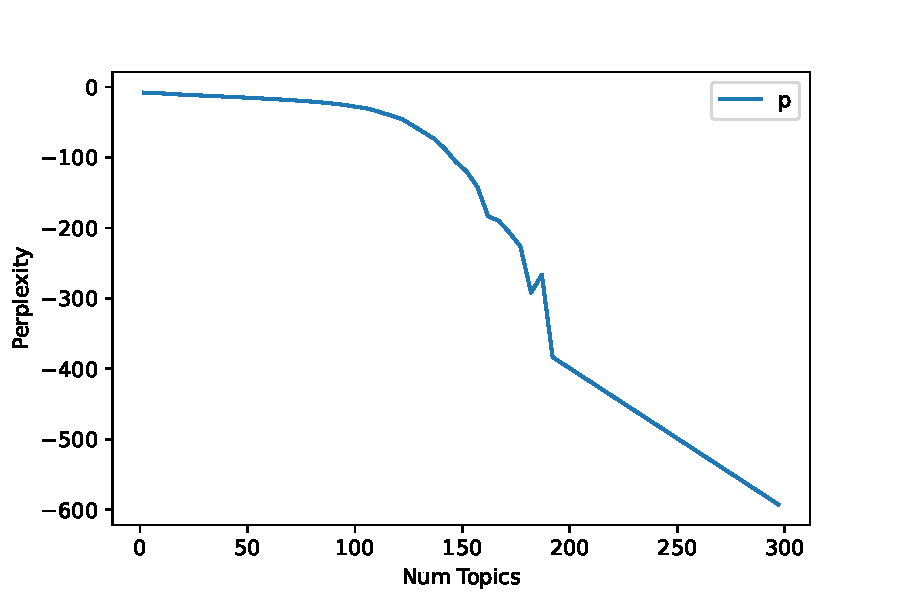
\includegraphics[width=\linewidth]{figures/topic_count}
	\caption{Perplexity of the LDA model over $k$}
	\label{fig:topiccount}
\end{figure}

Having a closer look into the similarity of topics within the model seem to confirm this impression. Fig. \ref{fig:topic-dissim} shows the dissimilarity of topics within the model build from tweets of democrats. A low score (red) means topics are similar, while a high score (blue) indicate a high dissimilarity. From this perspective \ref{fig:k15} is more desirable than \ref{fig:k130}.

\begin{figure*}
	\centering
	\begin{subfigure}[b]{0.45\textwidth}
		\centering
		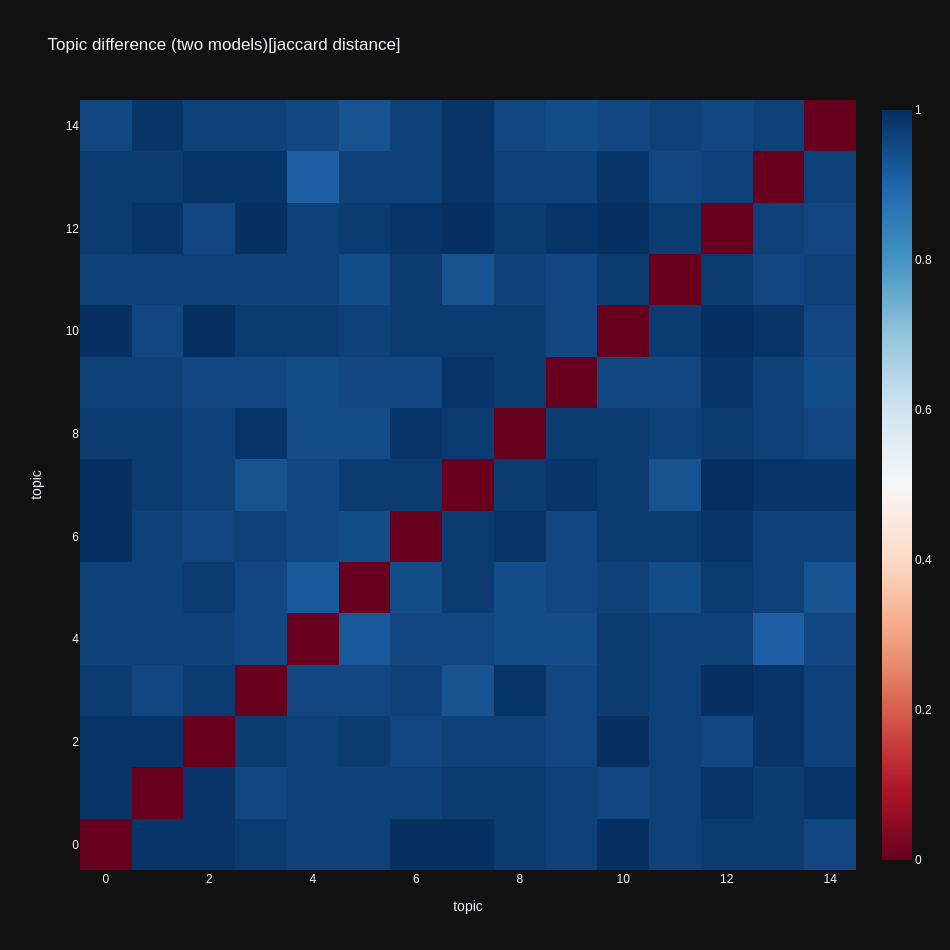
\includegraphics[width=\textwidth]{figures/dem_dem_diff_15.png}
		\caption{$k=15$}
		\label{fig:k15}
	\end{subfigure}
	\hfill
	\begin{subfigure}[b]{0.45\textwidth}
		\centering
		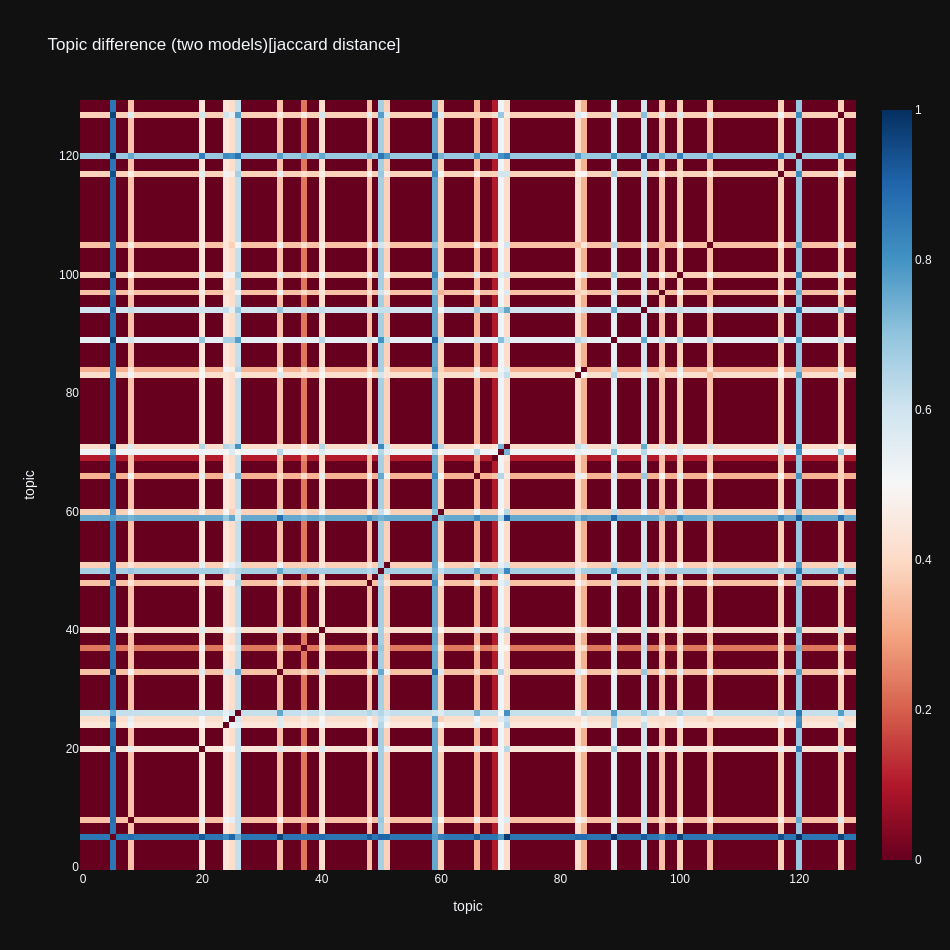
\includegraphics[width=\textwidth]{figures/dem_dem_diff_130.png}
		\caption{$k=130$}
		\label{fig:k130}
	\end{subfigure}
	\caption{Pairwise dissimilarity of topics build from tweets of Democrats}
	\label{fig:topic-dissim}
\end{figure*}

\begin{figure}
	\centering
	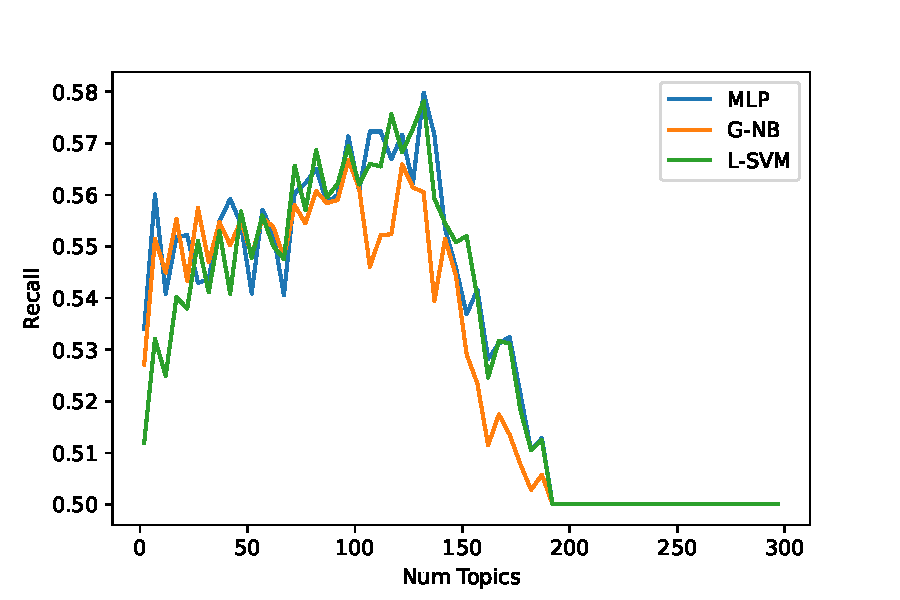
\includegraphics[width=\linewidth]{figures/topic_recall.pdf}
	\caption{Recall over $k$}
	\label{fig:rec}
\end{figure}

\begin{figure}
	\centering
	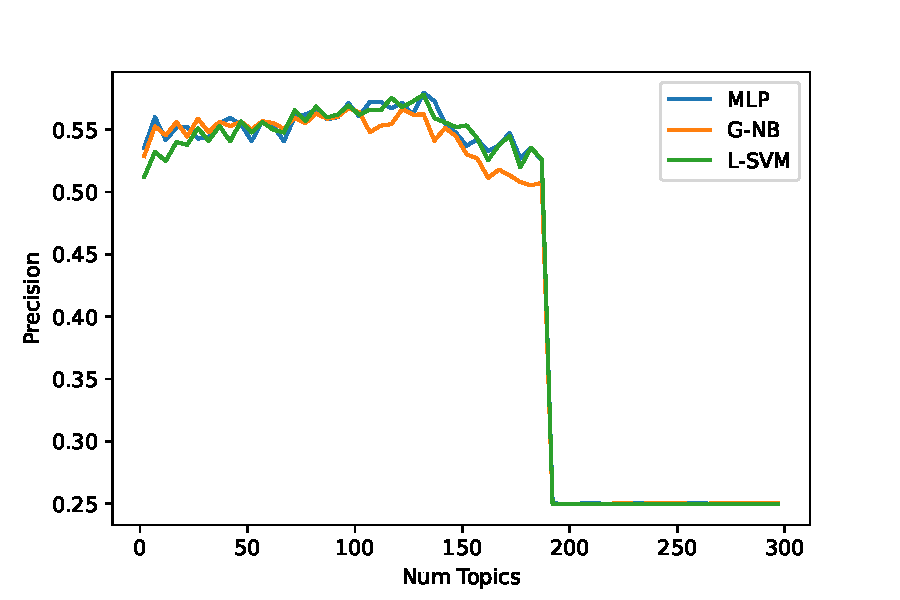
\includegraphics[width=\linewidth]{figures/topic_precision.pdf}
	\caption{Precision over $k$}
	\label{fig:pre}
\end{figure}

\begin{figure}
	\centering
	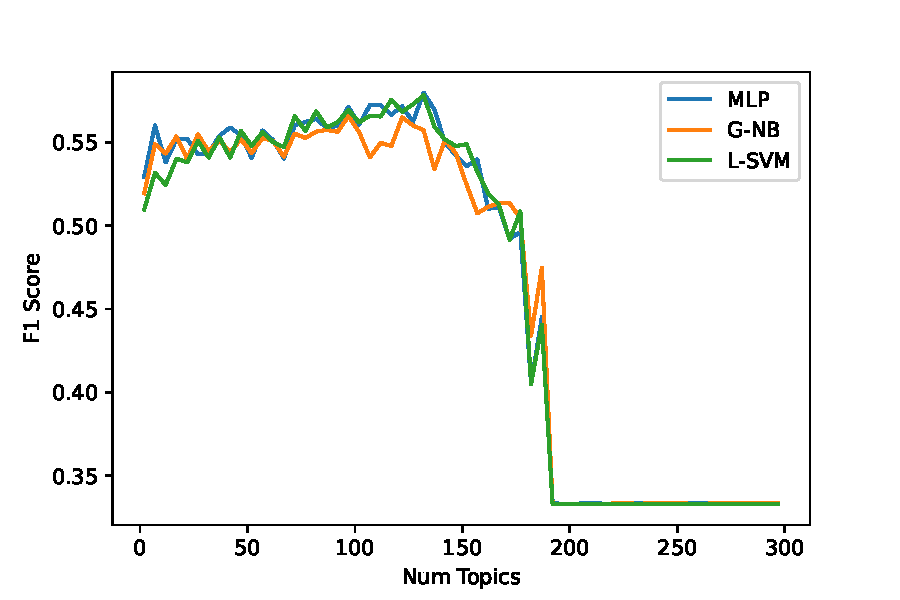
\includegraphics[width=\linewidth]{figures/topic_fscore.pdf}
	\caption{F$_1$-Score over $k$}
	\label{fig:f1}
\end{figure}

However, when measuring the overall performance of the classifier train using the respective model build with $k$ topics, we get contradictory results. We can observe in Fig. \ref{fig:rec}, \ref{fig:pre} and \ref{fig:f1} that for all three classifiers recall, precision and F$_1$-Score do not reach its peak at $k=15$. On the contrary, we see that all scores seem to find an optimum at $k=130$.

While we can observe that both Linear-SVM and Multi-Layer Perceptron are very similar in terms of their performance on the dataset, Gaussian Naive Bayes performs worse than the mentioned two above.

\begin{figure}
	\centering
	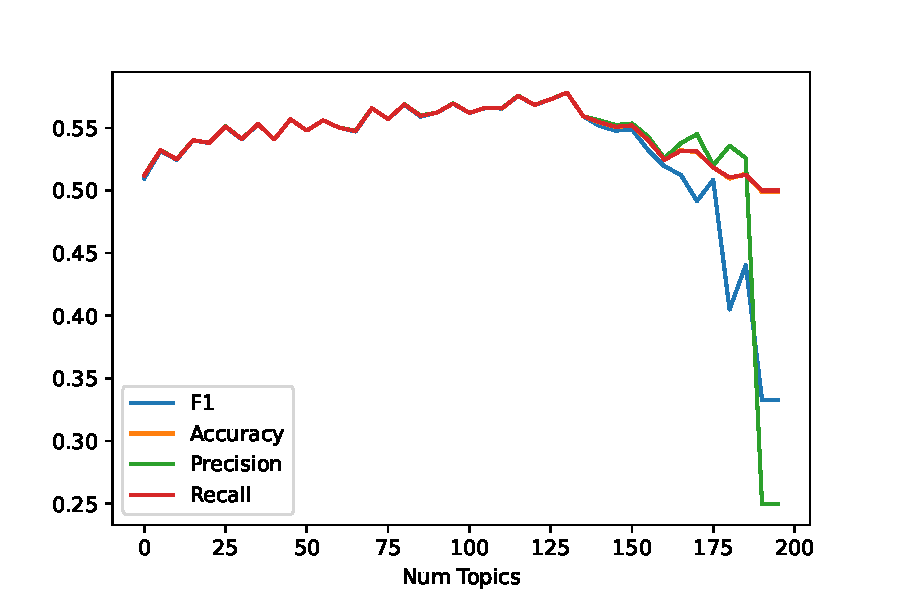
\includegraphics[width=\linewidth]{figures/summary_l-svm.pdf}
	\caption{Performance of L-SVM}
	\label{fig:sum-lsvm}
\end{figure}

\begin{figure}
	\centering
	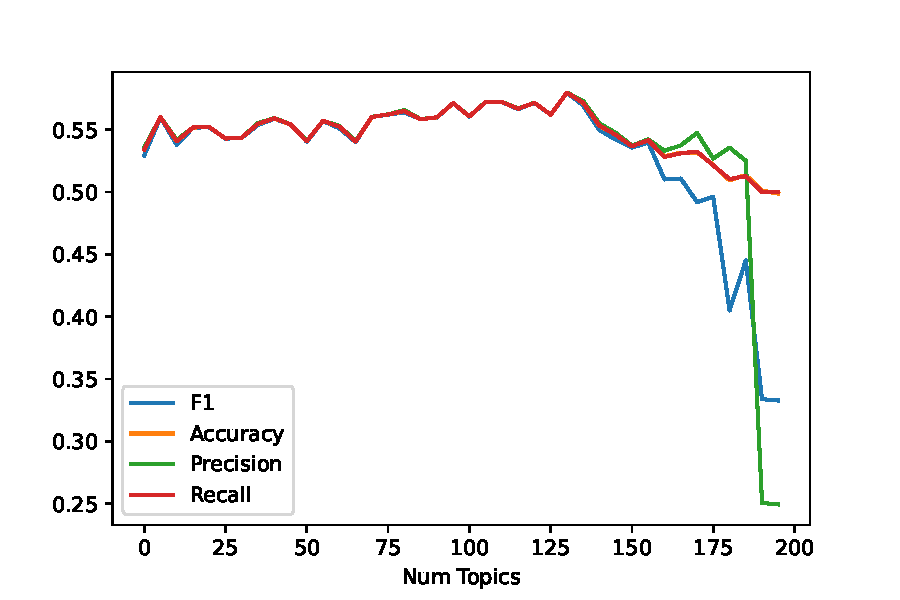
\includegraphics[width=\linewidth]{figures/summary_mlp.pdf}
	\caption{Performance of MLP}
	\label{fig:sum-mlp}
\end{figure}

If L-SVM and MLP are compared more closely together, we can spot a slightly better performance of L-SVM at $k=130$ as Fig. \ref{fig:sum-lsvm} and \ref{fig:sum-mlp} suggests.

Nevertheless, it is also clear that the results are not promising. At a peak the F$_1$-Score of 0.565 can only be archived, which is does not gives enough confidence to give reliable predictions on a users political view merely based on the users tweets.

\section{Summary}
\label{sec:summ}
To conclude the results of this approach it is obvious, that topic modeling using LDA-models do lead to the desired results such that no reliable predictions of the political view of users based on their tweets can be made.

Therefore, it seems that unsupervised, generative LDA models are unable to capture semantic meaning towards certain, for the political position relevant topics by just using statistical methods.

Further work could investigate, whether supervised methods, especially Deep Learning are better solutions to this task. E.g. one may fine tune existing and overall well performing transformer models such as BERT for this classification task.

%\clearpage

\bibliographystyle{ACM-Reference-Format}
\bibliography{sample}

\end{document}
\endinput
